\documentclass[12pt,letterpaper,fleqn]{article}

\usepackage[top=1in,bottom=1in,left=1in,right=1in]{geometry}
\usepackage{multicol}
\usepackage{graphicx}
\usepackage{pdfpages}
\usepackage{amsmath}
\usepackage{verbatim}
\usepackage[margin=10pt,font=normal,labelfont=bf]{caption}
\usepackage{empheq}
\usepackage{hyperref}
\usepackage{longtable}

\newcommand*\widefbox[1]{\fbox{\hspace{2em}#1\hspace{2em}}}
\newcommand{\dC}{^{o}C}
\newcommand{\HRule}{\noindent\rule{\linewidth}{0.5mm}}

\newcommand{\spc}[2][l]{%
  \begin{tabular}[#1]{@{}l@{}}#2\end{tabular}}

\setlength{\parindent}{0in} % No indentation
\setlength{\parskip}{0.5cm}
\setlength{\tabcolsep}{4pt} % Tight table

%\setcounter{secnumdepth}{2}

%\renewcommand{\includegraphics}[2][]{} % To ignore figures
%\renewcommand{\caption}[1]{} % To ignore captions

\begin{document}

\begin{titlepage}
  \begin{center}

    \HRule \\[0.4cm]

    \textsc{\LARGE Guam Renewable Integration}\\[0.2cm]
    \textsc{\large ENERGY 291 Final Project}
    
    
    \HRule \\[1.5cm]

    \begin{minipage}{0.45\textwidth}
      \begin{flushleft} \large
        \emph{Authors:}\\
        Martin \textsc{Chang}\\
        Ryan \textsc{Satterlee}
      \end{flushleft}
    \end{minipage}
    \begin{minipage}{0.5\textwidth}
      \begin{flushright} \large
        \emph{Professor:}\\
        Adam \textsc{Brandt}\\%[3cm]
        \emph{}
      \end{flushright}
    \end{minipage}

    \vfill
    {\large \today}

  \end{center}
\end{titlepage}

\section{Introduction}

High electricity prices on island nations and territories result from
a limitation of conventional energy resources, necessitating the
expensive imports of primarily liquid fuels by sea. The potential for
cheaper systems exists through a combination of increased deployment
of renewable energy, energy storage, and optimal grid
planning. Additionally, reducing reliance on imported fuels increases
the robustness and resiliency of the grid system against fuel
shortages and price shocks.

In this report, we will investigate the optimization of grid planning
on the island of Guam, with a focus on minimizing net present value
costs of a system upgrade. This will involve simultaneously optimizing
two interdependent variables: (1) the quantity of new renewable energy
capacity to build and (2) the geolocation of these new systems, based
on recommended locations by NREL, resource availability, and
transmission costs.

Guam is currently serviced by a single utility, the Guam Power
Authority (GPA), which makes island-wide grid changes and planning
more feasible. GPA owns 552.8 MW of gross generation capacity, 663
miles of T\&D lines, and 29 substations \cite{gpa14a}. On an annual
basis, Guam consumes on the order of 2 billion kWh, generated by means
of petroleum products, primarily residual fuel oil (RFO \#6) and a
small amount of diesel (No. 2 distillate) used for peaking purposes
\cite{gpa14a, eia12}. This electricity comes at a cost of \$0.27/kWh
as of January 2012, or about 2.5 times that of the US
mainland. Additionally, Guam is considering exploring LNG as a
conventional alternative, and passed a renewable portfolio standard of
5\% by 2015 and 25\% by 2035 \cite{eia12}.

Although it is well accepted that there is the potential for
economically sound investments in new energy technologies,
particularly solar PV, on islands that import oil for electricity,
this project seeks to develop how this plan might be carried out and
to determine what the limiting constraints on the problem are.

\section{Methods}

The model is a nonlinear cost minimization. The nonlinearity arises
from discontinuties due to transmission costs, which are fully
incurred for a site upon first construction at that site. Other costs
include capital costs (a function of installed capacity), fixed
operation \& maintenance (O\&M) costs (a function of cumulative
installed capacity), and variable O\&M costs including fuel (a
function of dispatched generation).

%\begin{comment}
\subsection{Mathematical Form}

\textbf{Objective Function:}\\
\emph{Minimize total costs, discounted to present value.}
  \[\text{min} \quad  \sum_{s \in SITES}\sum_{t \in TIME}(C_{st}^T + C_s^Cx_{st}
  + C_s^FB_{st} + C_s^VD_{st}) / (1 + d)^t\]
  \textbf{Subject to:}

  RPS Goal:\\
  \emph{For each year, the sum of all dispatch in that year of
    renewables must be at least the sum of all dispatch times the RPS
    percentage for that year.}
  \[\forall y \in YEARS \sum_{r \in RENEWABLES}\sum_{t \in TIME} D_{rt} \ge RPS_y \times
  \sum_{s \in SITES}\sum_{t \in TIME} D_{st}\]

  Dispatch Limit:\\
  \emph{For each site and timestep, dispatched generation can be no
    more than cumulative installed generation at that site up to that
    time.}
  \[\forall s,t \in SITES, TIME: D_{st} \le B_{st}\]

  Availability:\\
  \emph{For each renewable site, dispatched generation can be no more
    that the avaialability of the resource over the installed
    capacity.}
  \[\forall r,t \in RENEWABLES, TIME: D_{rt} \le A_{rt}B_{rt}\]

  Load:\\
  \emph{For all timesteps, dispatch must match load.}
  \[\forall t \in TIME: \sum_{s \in SITES} D_{st} = L_{t}\]

  Capacity:\\
  \emph{For all renewables, cumulative installed capacity cannot
    exceed the maximum capacities for that specific site.}
  \[\forall r,t \in RENEWABLES, TIME: B_{rt} \le P_r^{max}\]

  Budget:\\
  \emph{For each year, total capital expenditures cannot exceed an
    annual budget.}
  \[\forall y \in YEARS: \sum_{s \in SITES}\sum_{t \in TIME} C_{st}^T
  \le C_{y}^B\]

  Positivity Constraints:\\
  \emph{For each site and timestep, installed capacity and dispatch
    must be non-negative.}
  \[\forall s,t \in SITES, TIME: x_{st} \ge 0\]
  \[\forall s,t \in SITES, TIME: D_{st} \ge 0\]
  
  \textbf{where:}\\
  {\setlength{\parindent}{-1em}
    $\quad x_{st}^{}$ is the Decision variable: instantaneous amount of resource to build [$MW$]\\
    $\quad D_{st}^{}$ is the Decision variable: dispatch [$MWh$]\\
    $\quad B_{st}^{}$ is the Defined variable: cumulative developed resource [$MW$]\\
    $\quad C_{s}^{F}$ is the Fixed O\&M Cost + Transmission Costs [$\$/MWh$]\\
    $\quad C_{s}^{C}$ is the Capital Cost [$\$/MW$]\\
    $\quad C_{st}^{T}$ is the Tranmission Capital Cost [$\$/MW$]\\
    $\quad C_{s}^{V}$ is the Variable O\&M Costs [$\$/MW$]\\
    $\quad C_{y}^{B}$ is the Annual Budget [$\$/yr$]\\
    $\quad L_{ht}^{}$ is the Load [$MWh$]\\
    $\quad S_{t}^{}$ is the RPS goal [$\%$]\\
    $\quad A_{st}^{}$ is the Resource availability [$MWh/MW$]\\
    $\quad P_{s}^{max}$ is the Maximum site capacity [$MW$]\\
    $\quad d$ is the Discount rate\\
    $\quad SITES$ is the set of all generation sites (Oil, Diesel,
    Solar, and Wind)\\
    $\quad RENEWABLES$ is the set of all renewable generation sites
    (Solar and Wind)\\
    $\quad TIME$ is the set of all timesteps\\
    $\quad YEARS$ is the est of all years (2015 - 2036)
  }
%\end{comment}


\section{Data}

Our project initially intended to start with a geospatial optimization
of renewable energy sites based on constraints of rewnewable energy
sources, costs associated with building and operating these plants,
and the impact of land features (such as slope, urban areas, etc.) on
the cost of new T\&D lines, similar to Richard S. Middleton's
\emph{SimCCS} and \emph{SimWIND} studies \cite{middleton09,
  phillips12}. However, the NREL \emph{Initial Technical Assessment
  Report} already covered this step \cite{misty}. In this assessment,
NREL identified 7 solar and 3 wind sites, based on features such as
land availability, slope, and resource availability, using ArcGIS and
in-person site analysis (See Figure~\ref{fig:sites}). The top
3 solar sites and all 3 of the wind sites were used as candidate
locations for our model. The top 3 solar sites were determined by
having the largest space available for generation, as well as lower-to-no 
transmission costs, and close accessibility by road. The three wind sites
were determined by NREL using observational data and site analysis,
with only one site (W2-Navy) having reliable met tower data.

\begin{figure}[!h]
  \centering
  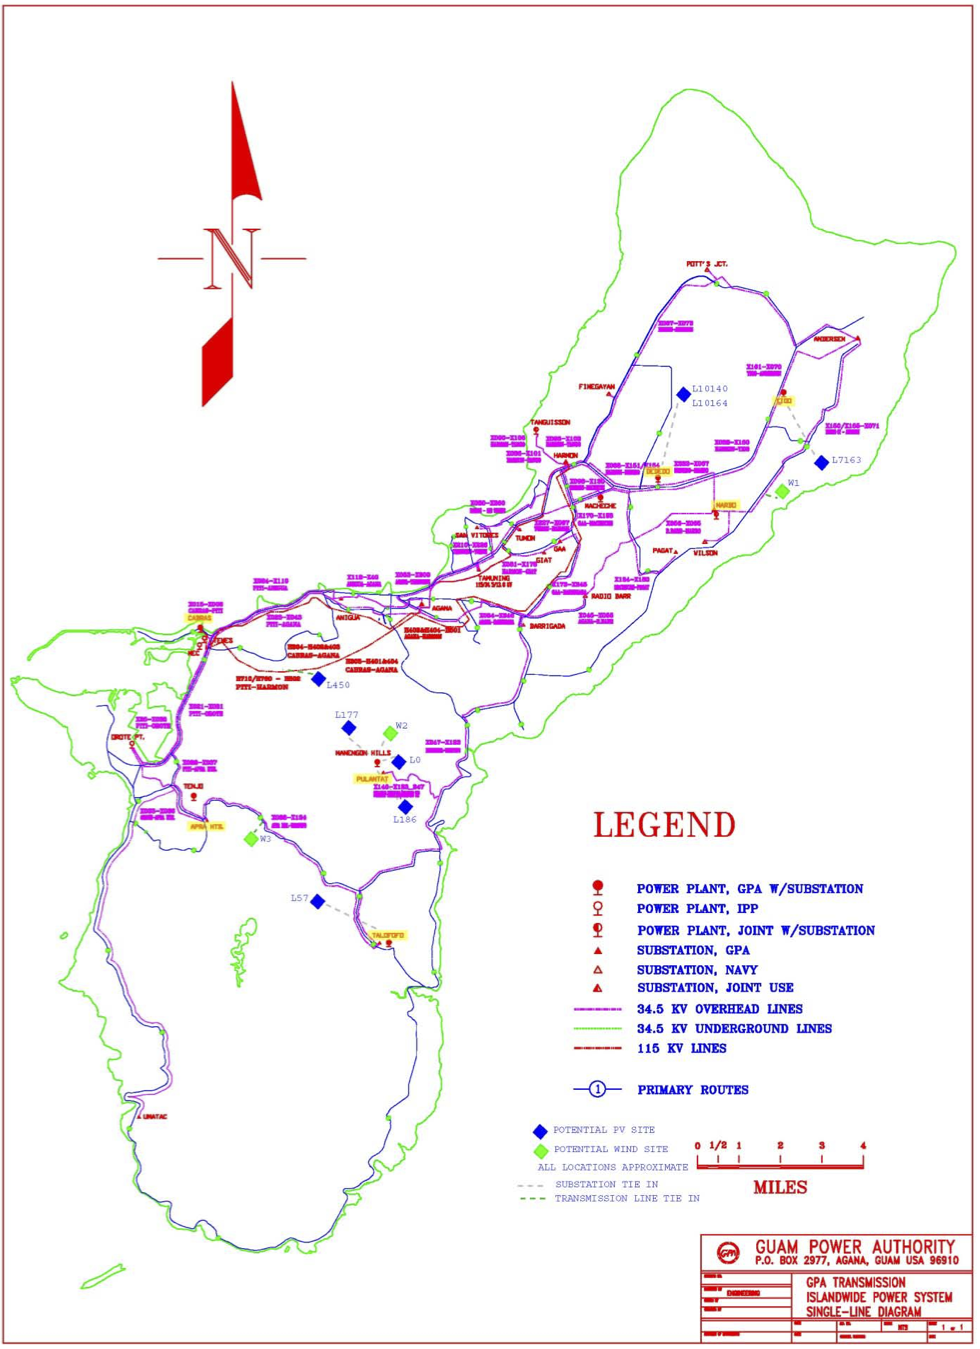
\includegraphics[width=0.925\textwidth]{img/sites}
  \caption{Candidate sites for solar and wind development identified by
    NREL.}
  \label{fig:sites}
\end{figure}

NREL provided access to two stations of TMY3 data that were used for
solar and wind resource mapping, although extrapolating radiation and
wind speed data from just two points is a source of innacuracy. An
additional 60m meteorological tower has been used for Naval wind
studies, providing a third, more accurate, assessment of wind resource
\cite{nrel09}. 

An important source of information for these data sets was the GPA. The GPA website gave access to a diagram of the
existing transmission lines, along with one-line diagrams showing the
electrical structure of the grid. GPA's 2008 and 2013 IRP give data on the
relevant features of the existing generation sources (nameplate
capacity, age, heat rates, operating costs, etc.) \cite{cruz08, cruz13}. Additionally, a
contact at GPA, Jennifer Sablan, provided the 2011-2013 hourly load
data \cite{sablan}.

See Table~\ref{tab:data} for a summary of all data sources.

%\begin{comment}
\begin{center}
  \begin{longtable}{| p{11cm} | p{3cm} | c | }
    \caption{Summary of Data Sources}
    \label{tab:data}\\

    \hline
    \multicolumn{1}{| l |}{\large{\textbf{Data} Description}} \rule{0pt}{3ex}& 
    \multicolumn{1}{c |}{\large{Value}} & 
    \multicolumn{1}{c |}{\large{Source}} %& 
    \\\hline\hline
    \endfirsthead

    \multicolumn{3}{c}
    {{\bfseries \tablename\ \thetable{} -- continued from previous
        page}} \\
    \hline
    \multicolumn{1}{| l |}{\large{\textbf{Data} Description}} \rule{0pt}{3ex}& 
    \multicolumn{1}{c |}{\large{Value}} & 
    \multicolumn{1}{c |}{\large{Source}}
    \\\hline\hline
    \endhead

    \multicolumn{3}{|r|}{{(\emph{Continued on next page)}}} \\ \hline
    \endfoot

    %\hline
    \endlastfoot

    \textbf{Solar and Wind Resource (TMY3)} Taken from the two sites
    located on Guam: Andersen Air Force Base, and Guam Weather
    Forecast Office (located at the Antonio B. Won Pat International
    Airport). Based on proximity, L450-R3 and L177-4-R2 were assumed
    to match the WFO and L7163 was assumed to match the AFB. Both
    W3-Cotal and W3-Pulantat were assumed to be an average of WFO and
    the Naval Base (below). 
    & Not attached, available online from NREL RReDC 
    & NREL \cite{nrel05} 
    \\\hline

    \textbf{Wind Resource (Naval Base)} Taken from a 60m meteorogical
    tower on a U.S. Naval Base. This resource was used for the site at
    W2-Navy and used with the TMY3-WFO data for W3-Cotal and
    W3-Pulantat 
    & Not attached, available online. 
    & Navy \cite{nrel09} 
    \\\hline

    \textbf{8760 Load Data} Hourly load from 2011-2013 was
    provided. In order to eliminate abnormalities inherent to each
    year, all three years were averaged into a single profile. This
    profile was then taken to be a more normal 2012, as the load had
    been steadily decreasing from 2011 to 2013, and 2012 was already
    close to being the average of the other two profiles. 
    & Not attached, available upon request 
    & GPA \cite{sablan} 
    \\\hline

    \textbf{Potential Solar and Wind Locations} Also includes distance
    to transmission for sites (L450-R3, L177-4-R2, L7163, L10140-R5
    and L10164-R3, L57-2, L0, L186NEW-1). 
    & \spc{See Figure~\ref{fig:sites};\\0 ft,\\370 ft,\\1200 ft,\\1600
    ft,\\2500 ft,\\850 ft,\\300 ft.}
    & NREL \cite{misty} 
    \\\hline

    \textbf{Existing Generation} Includes existing RFO, Diesel, and
    Solar on Guam. 
    & \spc{353.6 MW,\\199.2 MW,\\0.10906 MW}
    & NREL \cite{misty} 
    \\\hline

    \textbf{Maximum Allowable Generation} Includes solar sites
    (L450-R3, L177-4-R2, L7163, L10140-R5 and L10164-R3, L57-2, L0,
    L186NEW-1) and Wind (W3-Cotal, W3-Pulantat, W2-Navy). 
    & \spc{168.75 MW,\\160.8 MW,\\62.4 MW,\\28.65 MW,\\25.35
      MW,\\16.65 MW,\\10.8 MW,\\20 MW,\\10 MW,\\20 MW.}
    & NREL \cite{misty} 
    \\\hline

    \textbf{Costs for Solar} Includes capital, fixed and variable
    O\&M, and fuel. For a 20MW Utility PV facility, fixed tilt. 
    & \spc{\$4,183/kW,\\\$27.75/kW-yr,\\\$0/kWh,\\\$0/kWh\\(2013\$)}
    & EIA \cite{eia13} 
    \\\hline

    \textbf{Costs for Wind} Includes capital, fixed and variable O\&M,
    and fuel. For a 100 MW wind farm. 
    & \spc{\$2,213/kW,\\\$39.55/kW-yr,\\\$0/kWh,\\\$0/kWh\\(2013\$)}
    & EIA \cite{eia13} 
    \\\hline

    \textbf{Costs for RFO} Includes capital, fixed and variable O\&M,
    and fuel. For an oil fired steam turbine (not combined cycle). 
    & \spc{\$600/kW,\\\$5.5/kW-yr,\\\$0.0013/kWh,\\\$0.04693/kWh\\(2000\$)}
    & Shaalan \cite{shaalan01} 
    \\\hline

    \textbf{Costs for Diesel} Includes capital, fixed and variable
    O\&M, and fuel. For an oil fired combustion turbine. 
    & \spc{\$170/kW,\\\$3.5/kW-yr,\\\$0.005/kWh,\\\$0.06865/kWh\\(2000\$)}
    & Shaalan \cite{shaalan01} 
    \\\hline

    \textbf{Costs for RFO and Diesel Fuel} Increasing fuel costs were
    taken from the GPA's 2013 IRP, as their forecasted fuel
    costs. This overrides the fuel values from Shaalan, and was done
    to get a more accurate cost of fuel on the island (which is
    typically higher). The same assumed heat rates were kept from
    Shaalan's text, in order to arrive at a \$/kWh value. GPA's
    forecast was extrapolated from the provided 2015-2031 data to
    2035. It was assumed Guam could continue to use high sulfur fuel
    oil for RFO. The resulting variable O\&M costs were then fitted
    with a linear trendline the equation for which was directly coded
    into AMPL. 
    & See attached. 
    & GPA \cite{cruz13} 
    \\\hline

    \textbf{Load Scaling Factors} Used the predicted load values of
    sales in MWh and peak demand in MW from 2012-2029 and 2012-2025
    respectively. Chose the EPA Delay forecast scenario, as per the
    GPA's choice of using it in their own IRP. Values beyond 2025 and
    2029 were extrapolated from the last few years of each curve, as
    each forecast ends with a very linear behavior. 
    & See attached. 
    & GPA \cite{cruz13} 
    \\\hline

    \textbf{Cost of transmission} Based on the costs from the NCEP for
    a 69 kV double circuit line, as it was the closest option to the
    34.5 kV line for transmission in Guam. While a 115 kV lines exist
    on the island, the GPA specifically called out renewables as
    connection to the 34.5 kV circuit. A double circuit was assumed
    for added flexibility. A 4x factor from the NCEP was used in
    increasing the cost for underground transmission lines. This was
    done based on the recent initiative by the GPA to switch their
    T\&D underground for added resiliency and reliability. 
    & \$287.87/ft (\$2004)
    & NCEP \cite{brown04} 
    \\\hline

    \textbf{Solar Capital Costs} An assumption was made that PV
    overnight capital costs would continue to decrease over time,
    even without accounting for discounting. A Northwest Power and
    Conservation Council presentation from 2013 gives a project cost
    estimate for a 20 MW solar PV system from 2012-2035.  
    & See attached. 
    & NW Council \cite{simmons13} 
    \\\hline

  \end{longtable}
\end{center}
%\end{comment}

A large amount of preprocessing of the data was required to
incorporate it into the model. The 2011-2013 load data from GPA was
averaged in order to create a model baseline year without the
fluctuations of each individual year. This was then extrapolated from
2015-2035 based on the load growth prediction from Guam's 2013 IRP,
under the EPA delay forecast scenario \cite{cruz13}. This scenario
accounts for one possible military build up scenario in Guam from 2015
to 2019, and was the forecast scenario the GPA picked for their IRP
analysis, out of a set of scenarios provided to them by a third party
energy firm \cite{cruz13}.

Solar and wind resource data were extrapolated from the limited
TMY3 data that was available and the single meteorological tower from the
Navy. For solar resource availability, this involved combining diffuse and direct radiation to
determine incident radation levels, which could then be converted into
``sun-hours.'' This calculation uses the equations from Chapter 14 of
the 2009 ASHRAE Handbook \cite{ashrae}. This relies on the latitude
and longitude from the TMY3 file, as well as the direct normal (DNI)
and direct horizontal (DHI) irradiance. Through a series of
calculations involving the hour angle, solar altitude, solar azimuth,
and surface incidence angle, one can find the total irradiance on a
surface at any given angle. The irradiance on the PV panels was
calculated for panels tilted at an angle equal to latitude, and facing
due south.

Anenometer readings were extrapolated to hub heights
using the power law, with a Hellman exponent, $\alpha$, of 0.2:
\[v_2 = v_1\left(\frac{h_2}{h_1}\right)^\alpha\] 
These wind speeds could then be used to determine outputs of a GE
2.5MW turbine based on its power curve, approximated with a Gaussian
curve \cite{ge}. Each wind and solar site was designated to be
represented by either one of the three measurement sites or an average
of two, based on its proximity. While more site-specific data would
obviously be needed before construction at these sites, this serves as
a rough estimate of the available resource, given data constraints.

All load and resource data was then binned into appropriately sized
timesteps. The final model involved timesteps of 168 hours (1
week). In extrapolating resource data from 2015-2035, a uniform
degree of randomness (5\%) was included to provide variation between
different sites and years. 

\section{Results}

The final end result of the model utilizes the following parameters:
\begin{itemize}
\item 8 total sites (1 oil aggregate, 1 diesel aggregate, L450-R3
  solar, L177-4-R2 solar, L7163 solar, W2-Navy wind, W3-Cotal wind,
  W3-Pulantat wind)
\item 7\% discounting on costs
\item +/- 5\% randomness on the resource availability input vectors
  for each renewable site
\item Load growth following the EPA Delay forecast scenario
\item No forced dispatch of renewables
\item Wind cost data from GPA
\item Decreasing solar PV capital costs over time
\end{itemize}

For added accuracy to real life performance, an additional budget
constraint was added:
\begin{itemize}
\item \$200 million annual budget for capital expenditures
\end{itemize}

The resulting graph (Figure~\ref{fig:dispatch_base_case}) follows the
step function of the RPS quite closely, with some exceptions, given
the budgetary limit on spending (See Table~\ref{tab:rps}). Due to the
budget limit, the model does at times preempt the RPS goal and build
renewables earlier on in anticipation of continuing to meet said
goals. This is especially noticeable in the way that the model
surpasses the 10\% limit without ever building to it exactly, instead
jumping from 8\% to 12\%. Also, in most runs, year 2034 plays a role
in the model's final build up to 25\% renewables for 2035.

%\begin{comment}
\begin{table}[!h]
  \begin{center}
    \begin{tabular}{| c | c | c | }
      \hline
      \textbf{Year} & \textbf{RPS Goal} & \textbf{Modeled Renewable
        \%} \\\hline
      2015 & 5\% & 5\% \\\hline
      2016 & 5\% & 5.2\% \\\hline
      2017 & 5\% & 5\% \\\hline
      2018 & 5\% & 5\% \\\hline
      2019 & 5\% & 5.1\% \\\hline
      2020 & 8\% & 8\% \\\hline
      2021 & 8\% & 8.1\% \\\hline
      2022 & 8\% & 8.2\% \\\hline
      2023 & 8\% & 12.5\% \\\hline
      2024 & 8\% & 12.3\% \\\hline
      2025 & 10\% & 12.3\% \\\hline
      2026 & 10\% & 12.2\% \\\hline
      2027 & 10\% & 12.1\% \\\hline
      2028 & 10\% & 12.1\% \\\hline
      2029 & 10\% & 12\% \\\hline
      2030 & 15\% & 15\% \\\hline
      2031 & 15\% & 15\% \\\hline
      2032 & 15\% & 15\% \\\hline
      2033 & 15\% & 15\% \\\hline
      2034 & 15\% & 16.3\% \\\hline
      2035 & 25\% & 25\% \\\hline
    \end{tabular}
  \end{center}
  \caption{Comparison of modeled \% of generation that is renewable
    and the GPA's RPS goals.}
  \label{tab:rps}
\end{table}
%\end{comment}

As shown in Figure~\ref{fig:installed}, the model prefers to only
construct renewables when needed, typically around the 5 year mark for
each RPS step increase. There are exceptions due to the budget as
mentioned earlier, however. It can also be seen that the model favors
constructing two of the wind resources immediately and to
approximately maximum capacity first. This is likely due to the
foresight of the model recognizing the need for both wind and solar
later in the study period, due to the rising RPS, and optimizes
spending on wind first as it has a static capital cost. With solar
becoming cheaper with time, it is more advantageous to construct it as
late as possible. Additionally, while the L7163 is the smallest in
terms of maximum allowable capacity of the three solar sites, it is
constructed first. While the L450-R3 site already includes the
existing solar generation of today, since it has no transmission cost,
it is essentially already constructed in the eyes of the model. Still,
the fact that L7163 is constructed prior to L177-4-R2, which has a
cheaper transmission cost, is of interest, and may be due to the fact
that the larger capacities of the L177-4-R2 (as well as L450-R3) mean
larger quantities of cheaper solar can be built later on if the model
chooses to build the more expensive L7163 site first.

\begin{figure}[!h]
  \centering
  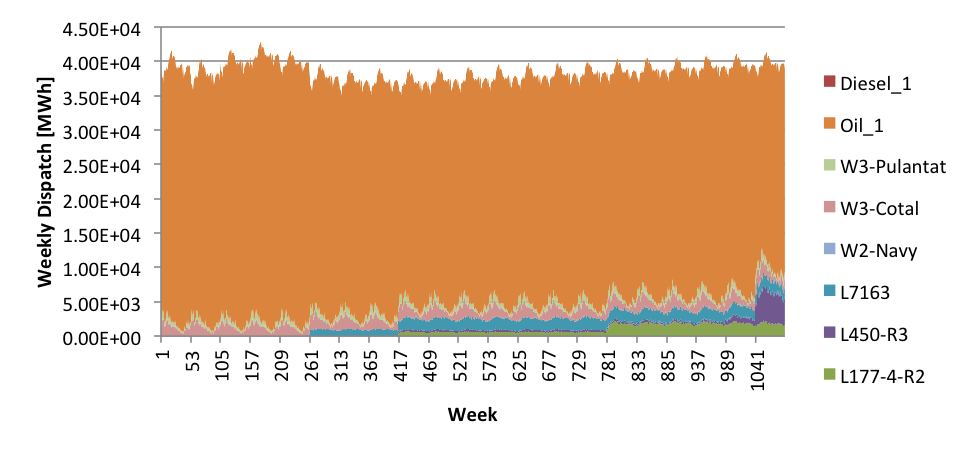
\includegraphics[width=0.9\textwidth]{img/dispatch_base_case}
  \caption{Weekly dispatch of \$200 M budget base case.}
  \label{fig:dispatch_base_case}
\end{figure}

\begin{figure}[!h]
  \centering
  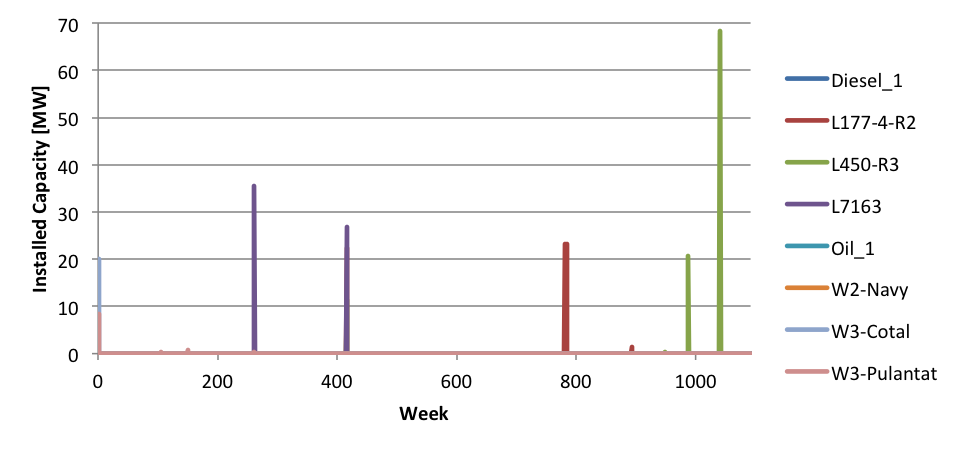
\includegraphics[width=0.9\textwidth]{img/installed}
  \caption{Installed capacity per week of \$200 M budget base case.}
  \label{fig:installed}
\end{figure}

In previous runs, the model would favor building the W2-Navy wind site
in the final year, as part of the large push to 25\%. However, the
dropping PV prices and higher wind costs per GPA's IRP have moved the
optimal solution to building more of the solar at existing sites,
rather than construct a new transmission line and fill in a new wind
resource site. 

The weekly dispatch performs reasonably well. As expected, the
majority of the generation is still fossil fuels, in this case, the
RFO baseload generation. Given the weekly time step required for
timely execution of the model, diesel generation is essentially
lost. This is because the diesel combustion turbine and medium speed
reciprocating engines serve the role of peaker plants, whose
importance is lost once on a time scale of weekly total dispatch. The
step increases of the RPS are quite evident in the resulting dispatch,
though it can be seen that more solar generation is built by week 417
(year 2023), prior to when it is needed in 2025. 

Although it is not immediately obvious from
Figure~\ref{fig:dispatch_base_case}, the increase in load under the
EPA delay forecast scenario does not seem to have a profound effect on
the system as a whole, as no real surplus generation is created to
meet the temporary increase in load. The RPS is still maintained
throughout the period, in part due to having been slightly oversized
for the previous years, as well as possibly in part due to the
coincident increase in randomness for wind variability. It is
interesting that the model chooses to construct solar at L177-4-R2
before filling in the already constructed L450-R3. This is in part due
to the budget constraint, as it is enough to allow for a more sharp
increase in generation each year). Additionally, the formulation of
the problem, with a fixed budget each year with decreasing PV costs,
discourages a gradual build up on sites before constructing the next
one. More details regarding the sensitivity of the model to the annual
budget set is available in the following section.

From this run, a final objective value of \$11,564,900,000 was
obtained. This totals to around \$550,709,524 per year, which is not
too far off from what the GPA can afford. As this cost covers new
construction and operation and maintenance of existing generation, it
is quite close to the actual annual fiscal budget of the GPA, which
was \$400.6 million in 2012 and \$413.5 million in 2013
\cite{cruz13}. Given the simplicity of the model, as well as the
assumptions that were made given the project timeline, a more accurate
model for GPA resource planning could be possible with continued fine
tuning.

\section{Senstivity/Uncertainty}

Since no single source had all costs for each of the sites (capital,
O\&M, fuel, transmission), costs were taken from various sources
instead. As a result, there are multiple instances of differing cost
numbers for various technologies. One staggering difference lies in
capital costs of onshore wind, between the numbers provided by the EIA
in 2013, and those by GPA in planning their IRP in 2012-2013
\cite{eia13, cruz13}. The EIA numbers were originally used at the
start of the project as it contained numbers for both solar PV and
wind. Additionally, it was one of the more recent sources for such
data available. However, upon closer inspect, the costs are based on
an assumed 100 MW site, whereas the sites to be built in Guam are
10-20 MW in size. Also, while the EIA does offer regional cost
adjustment factors to their numbers, it is restricted to electricity
regions on the continental U.S., and does not even have factors for
Hawaii, which would have been a more suitable substitute for
Guam. While solar PV capital cost data is now being taken from the NW
Council, wind data is still being taken from the EIA
\cite{simmons13}. The GPA have their own estimated costs for wind
projects in their territory, and the capital and fixed O\&M costs
differ from that of EIA by approximately twofold: 2013 \$2,213/kW
compared to 2012 \$4,650/kW, 2013 \$39.55/kW-yr compared to 2012
\$50/kW-yr \cite{eia13, cruz13}. The sensitivity of the end results to
this change in capital costs were tested by comparing runs with each
set of wind costs inputted. This case was run with a \$200 million
annual budget limit on capital construction, using the EPA-delay
scenario for load growth, +/- 5\% randomness for renewables,
discounting at 7\%, and declining PV prices to 2035.

In the EIA run (Figure~\ref{fig:cost_eia}), the model utilizes the
budget to construct solar at L7163 in 2019, prior to the 2020 RPS
increase. Both the W3-Cotal and W3-Pulantat sites are fully utilized
in terms of allowable installed capacity very early on. W2-Navy is
only constructed later to make the final push to 25\% in 2035. In
comparison, with the more expensive GPA wind cost data
(Figure~\ref{fig:cost_gpa}), the model never builds wind at W2-Navy,
and makes up for that difference with the now comparatively cheaper
solar PV at L177-4-R2. It is worth noting both models still start with
maximizing the two W3 wind sites, but this may not necessarily be a
cost matter directly. Rather, it is due to having perfect foresight
about future requirements, and the differences in wind and solar
resource availability.

Interestingly, with the more expensive wind set up, the total cost
across all 21 years is lower than that of the cheaper EIA wind data,
seeing \$11,979,200,000 instead of \$12,033,000,000. The difference is
relatively small, but since the difference is due to using more solar
at a site that will be constructed in either case, and from foregoing
the one-time transmission construction cost for the W2-Navy site, the
data suggests the current final objective function value from the EIA
data is not the global minimum. The EIA case should be able to reach
the same end values as the GPA case, and have an even lower final
objective value, since the only difference is the EIA case having
cheaper wind cost data.

\begin{figure}[!h]
  \centering
  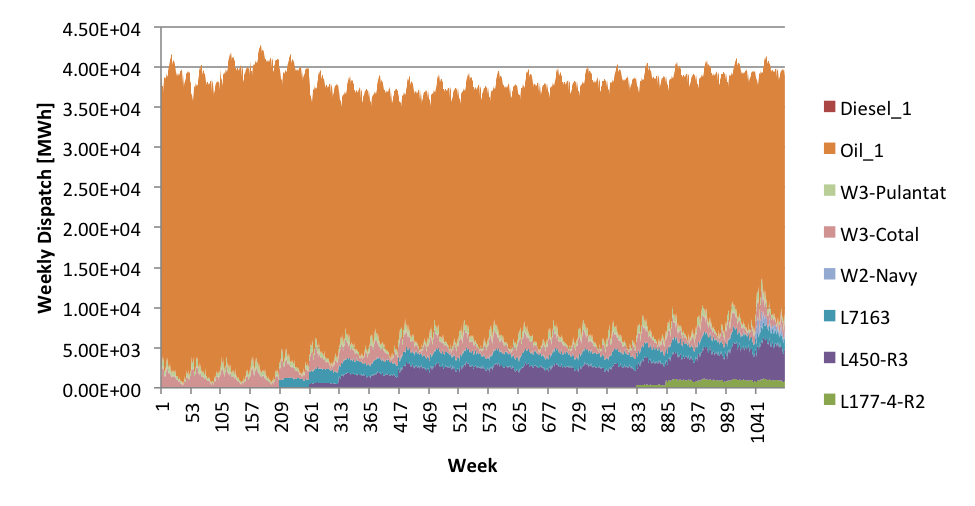
\includegraphics[width=0.9\textwidth]{img/cost_eia}
  \caption{Run using EIA cost assumptions.}
  \label{fig:cost_eia}
\end{figure}

\begin{figure}[!h]
  \centering
  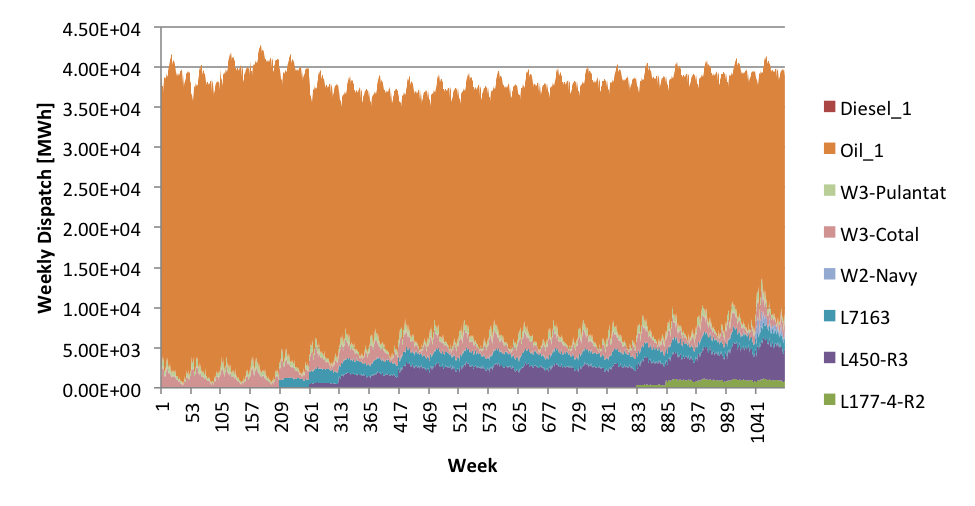
\includegraphics[width=0.9\textwidth]{img/cost_gpa}
  \caption{Run using GPA cost assumptions.}
  \label{fig:cost_gpa}
\end{figure}

Another large assumption in the model was setting an annual
budget. The initial simplified model allowed for unlimited expenses to
meet the demand and RPS simultaneously. However, in order to push for
more realism, an annual budget constraint was added, as previously
mentioned. This budget, which was chosen as being half of the fiscal
year budget for the GPA in 2012, is not necessarily the best
assumption. The sensitivity of the model to this value was
tested. When set to both \$100 million and \$150 million annually, the
optimal solution was not reached, and instead the nonlinear
infeasibilities were minimized by AMPL. The model behavior differed
from that expected, and constructed RFO generation at the start of the
21 year period, then proceeded to only use diesel generation instead
of RFO. Additionally, especially odd behavior could be seen where the
model chose to use large amounts of diesel, and then proceeded to
curtail all renewables for certain portions of each year, as seen in
Figure~\ref{fig:budget_100_not_forced}.

\begin{figure}[!h]
  \centering
  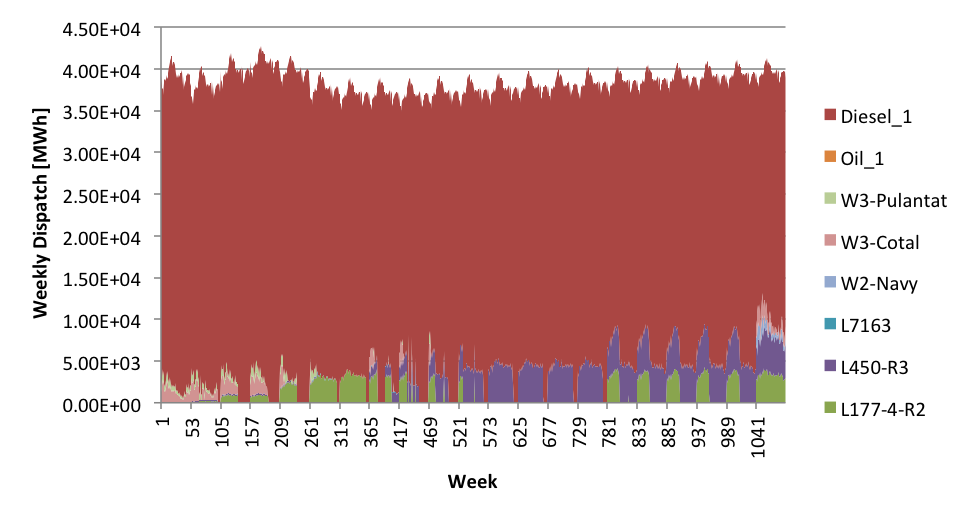
\includegraphics[width=0.9\textwidth]{img/budget_100_not_forced}
  \caption{\$100 M budget run with curtailment evident.}
  \label{fig:budget_100_not_forced}
\end{figure}

If renewable dispatch is explicitly enforced via constraint, then the
resulting system exceedes the RPS by the end of the 21 years,
upwards of 29.7\% (Figure~\ref{fig:budget_100_forced}). 
However, in this case Guam will also spend almost
\$8 billion more than the \$200 M budget case (regardless of whether
or not that case had renewable dispatch forced), and the model again
chose to run diesel over oil, despite the more expensive operating
costs of diesel.

\begin{figure}[!h]
  \centering
  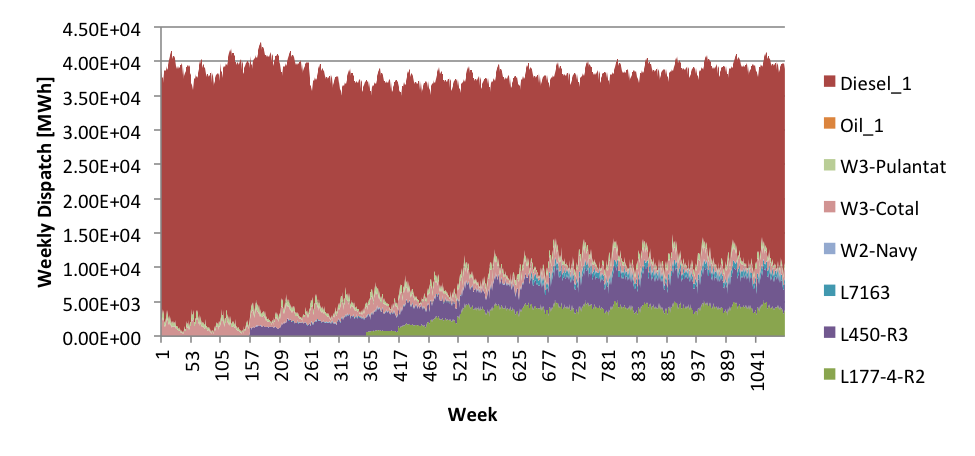
\includegraphics[width=0.9\textwidth]{img/budget_100_forced}
  \caption{\$100 M budget run with forced renewable dispatch and no
    curtailment evident.}
  \label{fig:budget_100_forced}
\end{figure}

On the other end of the spectrum, the higher the budget from the \$200
million, the closer the model performs to the original unlimited
budget case, as expected. With an increase to \$300 million annually,
the model already performs close to the unlimited form, with a
dispatch plot very closely matching the RPS
(Figure~\ref{fig:budget_300_not_forced}). In fact, the portion of
dispatch from renewables each year is exactly that of the RPS for that
year within 0.2\% of the load.

\begin{figure}[!h]
  \centering
  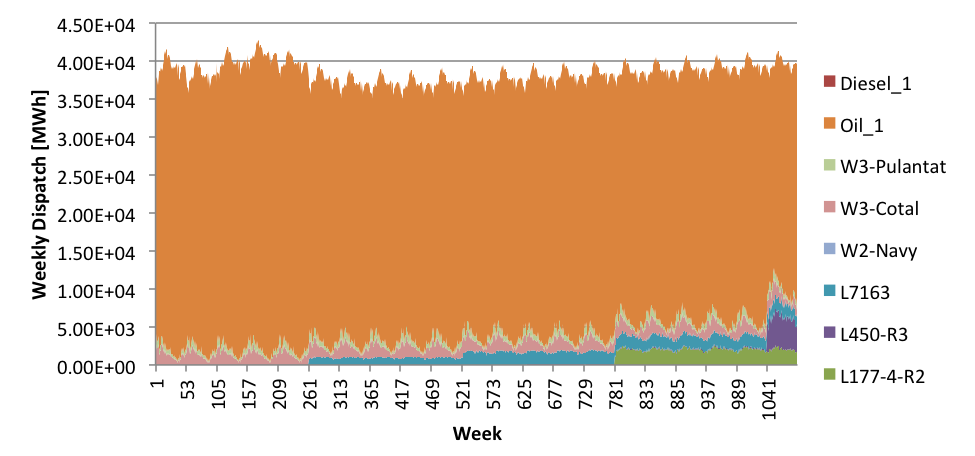
\includegraphics[width=0.9\textwidth]{img/budget_300_not_forced}
  \caption{\$300 M budget run with no forced dispatch of renewables.}
  \label{fig:budget_300_not_forced}
\end{figure}

It would appear the chosen \$200 million is not an unreasonable 
assumption, and is also near the minimum of acceptable budget limits,
before the model begins to behave abnormally by curtailing renewables
and excessively using peaker plants as baseload
generation. Additionally, the larger the budget, the less total cost
is spent on meeting the RPS. For example, the \$300 million budget run
has a total cost of \$11,338 million, while the \$200 million budget
run has a total cost of \$11,565 million.

\section{Discussion}

As was expected at the onset of the project, the sheer amount of data
was the primary barrier in determining an optimal model that would
feasibly solve in a reasonable amount of time. Integration of
renewables under an RPS is a problem that requires both a large
longitudinal timeframe as well as small timesteps to accurately
represent the true system. We decided to prioritize the 21-year
timeframe, which considerably sacrificed in timestep, forcing weeklong
timesteps. An ideal model would reduce this to hour timesteps, or even
15 minutes. This would allow for better representation of the intermittencies 
of renewable generation, and would allow for peaker plants to play a proper
role in generation, rather than being made irrelevant as was done to diesel
in this study. Our current data set has many of the basic data needed for
one hour timesteps, including load and resource data. However, smaller
timesteps would also require additional data on timely effects such as
ramp rates of the fossil-based generation. 

Additionally, many heuristics were used to simplify the volume of data
required for the model. The most glaring of such assumptions was that the
resource at each solar and wind site could be approximated by the TMY3
data at one of two sites, or a simple average combination of the two
sites. A more accurate study would collect data specific to the
individual conditions of each proposed location.

The model also relies on many results of the NREL Assessment, some of
which are incomplete. For example, NREL determined the distances to
transmission lines for each candidate site, but costs for installing
this transmission were assumed to be linearly related to distance. In
reality, a more accurate model would depend on features of the land,
distance, and required capacity to determine local costs, as was done
in the \emph{SimWIND} study \cite{phillips12}. 

Having solid cost information became an issue, as much of it came from
such a varied array of sources, each with their own assumptions, and
almost all of which were specific to locations on the
U.S. mainland. This is particularly important as the higher cost of
burning fossil fuels due to the greater difficulty of obtaining them
on an island such as Guam is part of the basis for this study. Other
concerns would be higher construction costs on an island due to
greater difficulty with transportation as well. Inputting how these
costs change with time is similarly important, as they may all change
differently. Other cost data, such as tax incentives and more accurate
financing of capital investments, would also have helped establish
more realistic grounds for comparison between renewables and
conventional generation types. Finally, knowing the true GPA budget
for capital investments would have been better, although the current
assumption of \$200 million seems to hold up well in analysis, and in
the context of their total annual budget being on the order of \$400
million.

One factor that was not included that could have led to more realistic
results is a measure of construction time. Currently, the model is
allowed to construct sites in a single timestep (constrained by an
annual budget), which is obviously impossible. This is what leads to
the very ``chunky'' behavior of the resulting installation schedule,
as generation can be built as soon as it is needed. In a more
realistic scenario, some of the capacity may come online gradually as
solar arrays and wind turbines are erected.

In addition to construction contraints on timeslines, generation
lifetimes and retirements need to be accounted for. 
Upon closer investigation of the GPA's own plans for
retirement, it seemed the impact would be small as they only intended
to retire two diesel combustion turbines, for which they already have
excess capacity \cite{cruz13}. However, part of this retirement plan
assumed other older plants, namely baseload plants, would be converted
to natural gas fired versions, or assimilated into a combined cycle
system, also using natural gas.  If these plants were to be retired
completely instead, in favor of growing renewable penetration, it
would be pertinent to include this in the model.

Another aspect of the model that had to be left out was the potential
for energy storage. Besides the difficulties of cost assumptions,
storage was also made nearly impossible to integrate with the need for
large timesteps. With solar and wind resource data aggregated over
weeklong timesteps and multiple sites, any intermittancy is smoothed
out, leaving little room in the current model for energy storage to
provide value. Addressing the above points would serve to improve the 
model beyond it's current limitations, and create a more useful tool for 
Guam's resource planning in terms of accommodating more renewabls.

\begin{thebibliography}{99}

\bibitem{ashrae}
  American Society of Heating, Refrigerating and Air-Conditioning Engineers, Inc. (ASHRAE). 
  \emph{2009 ASHRAE Handbook - Fundamentals}. 
  Retrieved March 16, 2014 from
  \url{http://app.knovel.com/hotlink/toc/id:kpASHRAE22/ashrae-handbook-fundamentals-2}

\bibitem{misty}
  Baring-Gould, I. et al. (April 2011).
  \emph{Guam Initial Technical Assessment Report}.
  National Renewable Energy Laboratory (NREL).
  Retrieved from \url{http://www.nrel.gov/docs/fy11osti/50580.pdf}
  
\bibitem{brown04}
  Brown, Matthew H., and Richard P. Sedano (2004).
  \emph{Electricity Transmission, A Primer}.
  N.p.: National Council on Electric Policy.
  U.S. Departement of Energy.
  Retrieved March 16, 2014 from
  \url{http://energy.gov/oe/downloads/electricity-transmission-primer}

\bibitem{cruz08}
  Cruz, John J. (Aug 2008).
  \emph{Integrated Resource Plan, FY 2008}.
  Guam Power Authority.

\bibitem{cruz13}
  Cruz, John J., and Jennifer G. Sablan (Feb 2013).
  \emph{Integrated Resource Plan FY 2013}.
  Guam Power Authority.
  Retrieved March 16, 2014 from
  \url{http://guampowerauthority.com/gpa_authority/strategicplanning/2012IRP.php}

\bibitem{dsire}
  DSIRE (2012).
  \emph{Guam Renewable Energy Portfolio Goal}.
  Database of State Incentives for Renewable Energy.
  
\bibitem{ge}
  General Electric (GE).
  \emph{2.5MW Wind Turbine Series}.
  GE Power \& Water, Renewable Energy.
  Retrieved March 10, 2014 from
  \url{http://www.ge-energy.com/content/multimedia/_files/downloads/GEA17007A-Wind25Brochure.pdf}

\bibitem{gpa10}
  Guam Power Authority (2010).
  \emph{2010 GPA Met Tower Wind Data}.
  Retrieved March 3, 2014 from
  \url{http://guampowerauthority.com/special/documents/2010GPAMetTowerWindData.xls}

\bibitem{gpa14a} 
  Guam Power Authority.
  \emph{Fact Sheet}.
  Retrieved March 13, 2014 from: 
  \url{http://guampowerauthority.com/gpa_authority/about/gpa_fact_sheet.php}.

\bibitem{gpa08b}
  Guam Power Authority (2008).
  \emph{Generation Resource Handbook, FY 2008}.
  Retrieved from
  \url{http://guampowerauthority.com/gpa_authority/strategicplanning/documents/FY2008GenerationResourceHandbook.pdf}

\bibitem{gpa_trans}
  Guam Power Authority.
  \emph{GPA Transmission Islandwide Power System Single-Line Diagram}.
  Retrieved from 
  \url{http://guampowerauthority.com/gpa_authority/engineering/documents/IslandwidePlantsandTransmission.pdf}

\bibitem{middleton09}
  Middleton, Richard S. and Jeffery M. Bielicki.
  \emph{A scalable infrastructure model for carbon capture and
    storage: SimCCS}.
  Energy Policy 37.
  1052-1060.

\bibitem{nrel05}
  National Renewable Energy Laboratory (2005)
  \emph{National Solar Radiation Data Base}.
  Retrieved March 3, 2014 from
  \url{http://rredc.nrel.gov/solar/old_data/nsrdb/1991-2005/tmy3/}

\bibitem{nrel09}
  National Renewable Energy Laboratory (Jan 2009).
  \emph{Wind Resource Data Summary, Guam Naval Ordianance Annex}.
  Retrieved from
  \url{http://guampowerauthority.com/special/documents/GuamNavalOrdnanceAnnex-200911Summary.pdf}

\bibitem{phillips12}
  Phillips, Benjamin R. and Richard S. Middleton.
  \emph{SimWIND: A geospatial infrastructure model for optimizing wind
    power generation and transmission}.
  Energy Policy 43.
  291-302.

\bibitem{sablan}
  Sablan, Jennifer (Mar 2014).
  \emph{GPA 2011-2013 Hourly Load Data}.
  Guam Power Authority.
  Email Correspondence.

\bibitem{shaalan01}
  Shaalan, Hesham E. (2001).
  \emph{Generation of Electric Power}.
  Handbook of Electric Power Calculations.
  By H. Wayne. Beaty.
  3rd ed. New York: McGraw-Hill.
  8.1-.38.
  Print.

\bibitem{simmons13}
  Simmons, Steve (Jun 2013).
  \emph{Utility Scale Solar PV Cost}.
  Northwest Power and Conservation Council.
  Retrieved March 16, 2014 from
  \url{http://www.nwcouncil.org/media/6867216/GRAC_SolarPV_Cost_062012.pdf}

\bibitem{eia12}
  U.S. Energy Information Administration (2012).
  \emph{Guam Territory Profile and Energy Analysis}
  Retrieved January 24, 2014 from
  \url{http://www.eia.gov/countries/country-data.cfm?fips=gq}

\bibitem{eia13}
  U.S. Energy Information Administration (Apr 2013).
  \emph{Updated Capital Cost Estimates for Utility Scale Electricity
    Generating Plants}.
  Retrieved March 16, 2014 from
  \url{http://www.eia.gov/forecasts/capitalcost/pdf/updated_capcost.pdf}

\end{thebibliography}

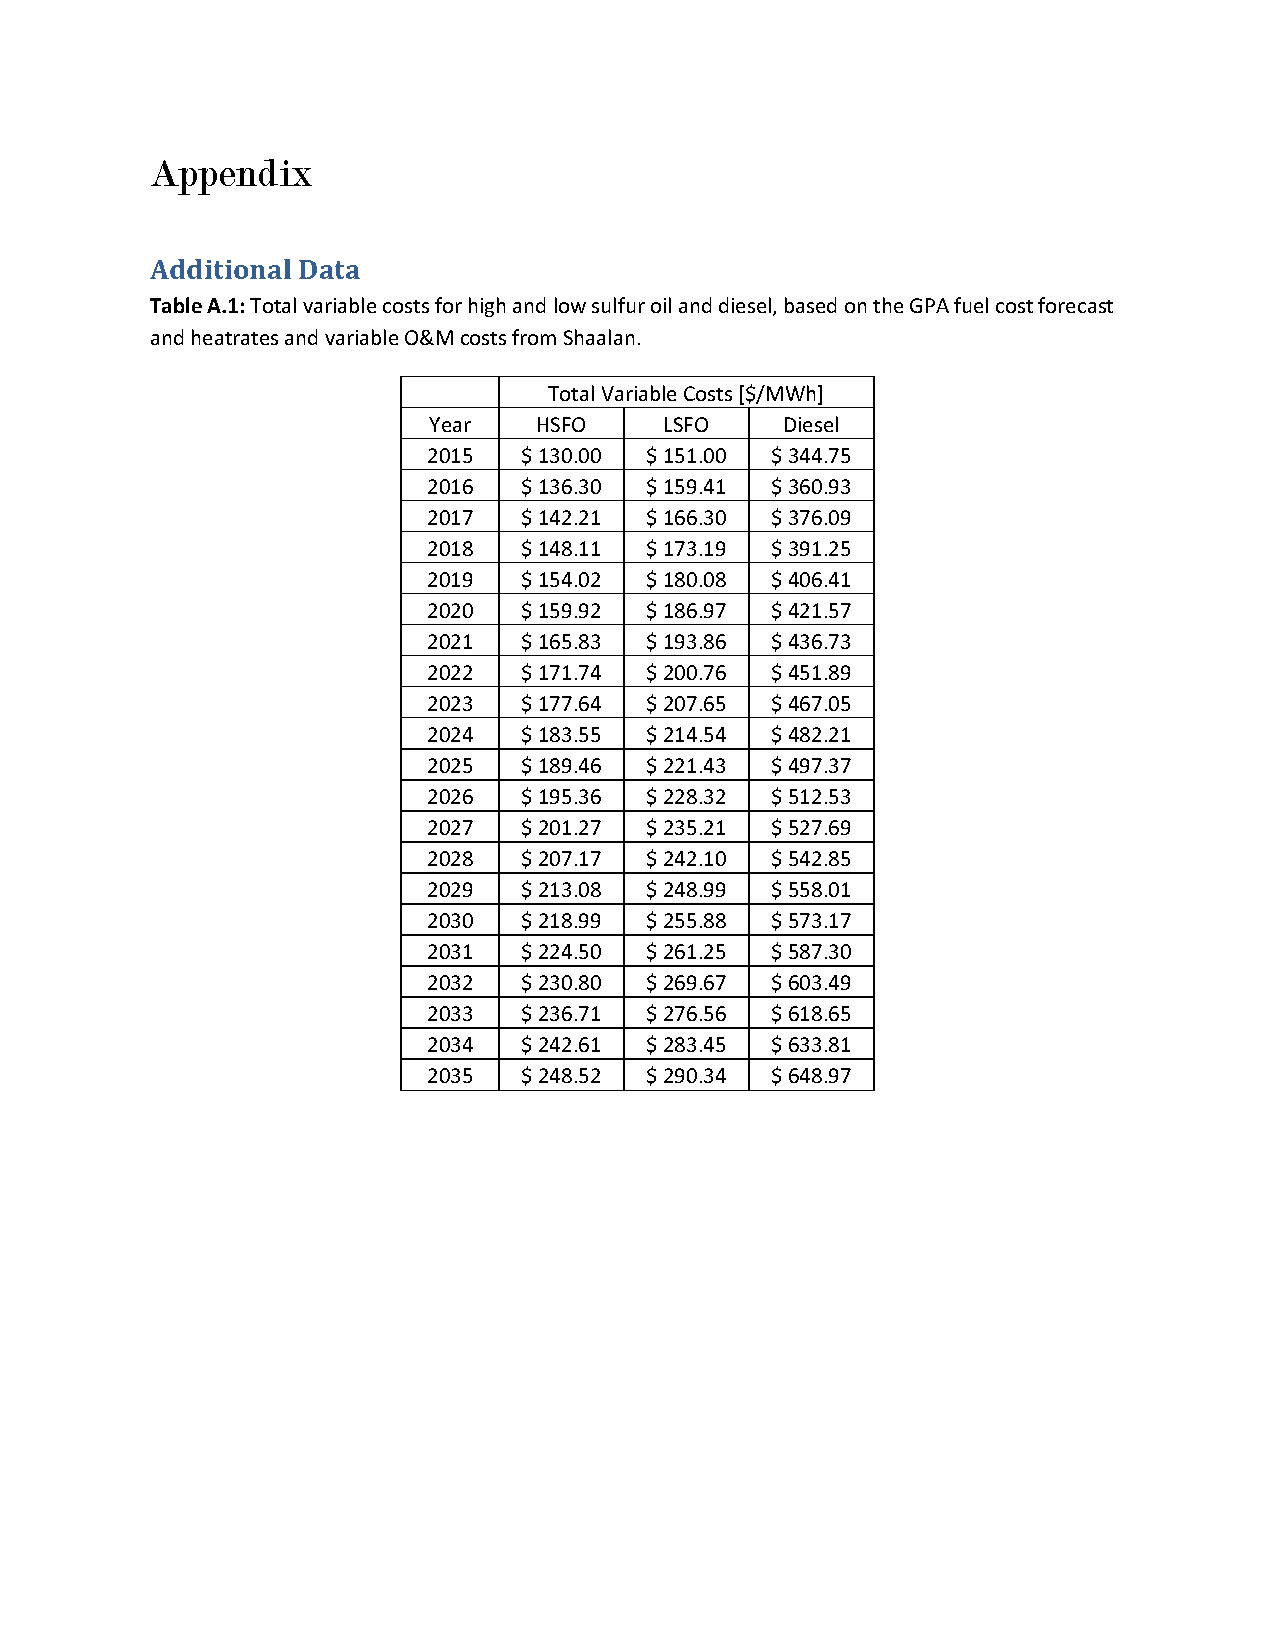
\includepdf[pages=-]{P5_Report_Appendix.pdf}

\end{document}